\thispagestyle{empty}
\global\watermarkfalse
\begin{tikzpicture}[remember picture,overlay]
  \coordinate (C) at (current page.center);
  % plain near-white page with one thin gilt rule
  \fill[ivory] (current page.south west) rectangle (current page.north east);
  \draw[gilt,line width=0.8pt] ($(current page.south west)+(0.6cm,0.6cm)$) rectangle ($(current page.north east)+(-0.6cm,-0.6cm)$);
  % top flourish and crest
  \node[inner sep=0pt] at ($(current page.north)+(0,-2.35cm)$) {\pgfornament[width=7cm,color=gilt]{87}};
  \node[inner sep=0pt] (crest) at ($(current page.north)+(0,-6.2cm)$) {
\includegraphics[width=6.2cm]{img/logo}};
  \draw[gilt,line width=1.2pt] (crest.center) circle (3.25cm);
  \draw[navy,line width=0.4pt] (crest.center) circle (3.4cm);
  % title block
  \node[align=center,text width=15cm] at ($(current page.north)+(0,-12.6cm)$) {%
    {\color{gilt}\scshape\large Science Monk \textperiodcentered{} Presents}\\[6pt]
    {\color{navy}\fontsize{46}{52}\selectfont\scshape NEET Physics}\\[4pt]
    {\color{ink}\fontsize{16}{20}\selectfont\itshape Previous Year Question Papers}\\[8pt]
    {\color{gilt}\pgfornament[width=5cm]{88}}\\[4pt]
    {\color{verde}\fontsize{15}{18}\selectfont\scshape 2016 \textendash{} 2026 \enspace\textperiodcentered\enspace Eleven Years \enspace\textperiodcentered\enspace 515 Questions}};
  % centre: calligraphic cartouche
  \coordinate (Q) at ($(current page.south)+(0,10.7cm)$);
  \begin{scope}
    \clip (Q) ellipse (6.9cm and 3.2cm);
    \fill[softgilt!35] (Q) ellipse (6.9cm and 3.2cm);
    % faint physics motifs
    \begin{scope}[shift={($(Q)+(-5.5cm,0.1cm)$)},gilt!55,line width=0.6pt]
      \draw (0,0) ellipse (1.3cm and 0.45cm);
      \draw[rotate=60] (0,0) ellipse (1.3cm and 0.45cm);
      \draw[rotate=-60] (0,0) ellipse (1.3cm and 0.45cm);
      \fill[navy!40] (0,0) circle (0.12cm);
    \end{scope}
    \draw[gilt!55,line width=0.6pt,domain=0:1.9,samples=80,shift={($(Q)+(4.4cm,-0.9cm)$)}] plot (\x,{0.35*sin(\x*240)});
    \draw[gilt!55,line width=0.6pt,domain=0:1.9,samples=80,shift={($(Q)+(4.4cm,-0.9cm)$)}] plot (\x,{0.35*cos(\x*240)});
  \end{scope}
  \draw[gilt,line width=1.6pt] (Q) ellipse (6.9cm and 3.2cm);
  \draw[gilt,line width=0.5pt] (Q) ellipse (6.7cm and 3.0cm);
  \draw[navy,line width=0.3pt] (Q) ellipse (7.05cm and 3.35cm);
  \node[inner sep=0pt,fill=ivory] at ($(Q)+(0,3.25cm)$) {\pgfornament[width=4.4cm,color=gilt]{88}};
  \node[inner sep=0pt,fill=ivory] at ($(Q)+(0,-3.25cm)$) {\pgfornament[width=4.4cm,color=gilt,symmetry=h]{88}};
  \node[inner sep=0pt] at ($(Q)+(-7.15cm,0)$) {\pgfornament[width=1.4cm,color=gilt,symmetry=v]{46}};
  \node[inner sep=0pt] at ($(Q)+(7.15cm,0)$) {\pgfornament[width=1.4cm,color=gilt]{46}};
  \node[align=center,text width=10cm] at ($(Q)+(0,0.25cm)$) {%
    {\color{navy}\fmmfamily\fontsize{36}{42}\selectfont The important thing}\\[2pt]
    {\color{navy}\fmmfamily\fontsize{36}{42}\selectfont is not to stop questioning}\\[8pt]
    {\color{gilt}\pgfornament[width=3.2cm]{88}}\\[1pt]
    {\color{crimson}\small\scshape Albert Einstein}};
  \node[align=center] at ($(current page.south)+(0,6.3cm)$) {%
    {\color{verde}\calligra\fontsize{20}{24}\selectfont every question retyped \quad every diagram redrawn}};
  % small square photo with name, bottom-left corner
  \node[inner sep=0pt,anchor=south west] (ph) at ($(current page.south west)+(4.4cm,2.6cm)$) {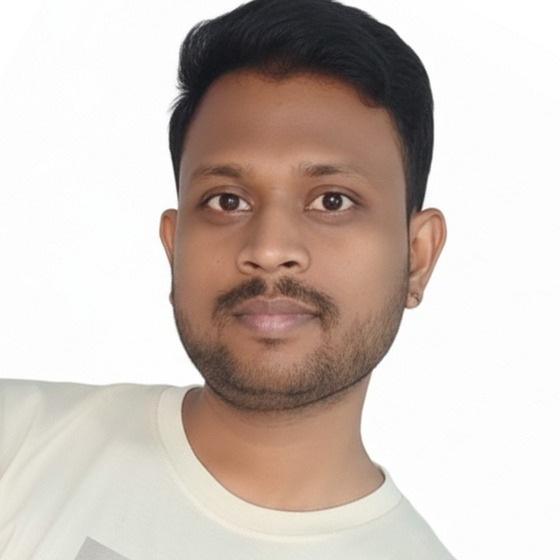
\includegraphics[width=2.4cm]{img/photo_square}};
  \draw[gilt,line width=1.2pt] (ph.south west) rectangle (ph.north east);
  \node[anchor=west,align=left] at ($(ph.east)+(0.35cm,0)$) {%
    {\color{navy}\fontsize{15}{18}\selectfont\scshape Sumeet Birajadar}\\[2pt]
    {\color{crimson}\small\itshape Founder \& Physics Mentor}\\
    {\color{ink}\small\scshape Science Monk}};
  \node[anchor=south east,align=right] at ($(current page.south east)+(-4.4cm,2.7cm)$) {%
    {\color{ink}\footnotesize\itshape\textquotedblleft Appa Deepo Bhava\textquotedblright}\\
    {\color{gilt}\footnotesize\scshape Learn \textperiodcentered{} Think \textperiodcentered{} Excel}};
\end{tikzpicture}
\null
\clearpage
\global\watermarktrue
